\chapter*{Lecture 26}
\begin{recall}{}{}
\begin{itemize}
\item Coupled systems
\item Register for the project!
\end{itemize}
\end{recall}




\subsection{Coupled Spring-Mass Systems}
Both masses are moving freely (friction and gravity are negligible) but they are now coupled:
\begin{figure}
\centering
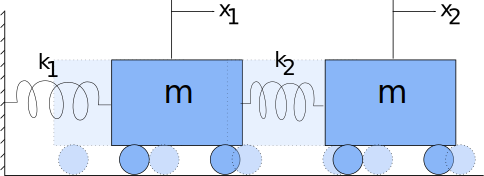
\includegraphics[width=0.6\textwidth]{figs/massSpringDamperSystemCoupled.pdf} 
\caption{Forced vibration with a coupled spring-mass system}
\end{figure}

\begin{itemize}
\item Force analysis:

\begin{figure}
\centering
\includegraphics[width=0.4\textwidth]{figs/massSpringDamperSystemCoupled_force1.pdf}
\caption{Mass 1}
\end{figure}
 \begin{figure}
\centering
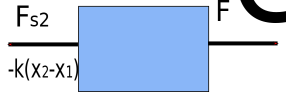
\includegraphics[width=0.4\textwidth]{figs/massSpringDamperSystemCoupled_force2.pdf} 
\caption{Mass 2}
\end{figure}

\item Newton's second law :
(Mass 1)
 \begin{align*}
m_1x''_1  = F_1+k_2\left(x_2-x_1\right)-k_1x_1
\end{align*}
by rearranging:
 \begin{align*}
\boxed{m_1x''_1 +\left(k_1+k_2\right)x_1-k_2x_2 = F_1}
\end{align*}
(Mass 2)
 \begin{align*}
m_2x''_2  = F_2-k_2\left(x_2-x_1\right)
\end{align*}
or
\begin{align*}
\boxed{m_2x''_2 +k_2x_2- k_2x_1= F_2}
\end{align*}
We need to solve a system of equations for $x_1$ and $x_2$

\item For the solution of this linear system of ODEs, we use \textbf{Gaussian elimination}
\end{itemize}





\subsection{Gaussian elimination}
For a system of 1st order ODEs:
\begin{align*}
a_1x'+a_2x+a_3y'+a_4y=f_1\\
a_5x'+a_6x+a_7y'+a_8y=f_2
\end{align*}
We introduce the differential operator:
\begin{align*}
D=\frac{d}{dt}\qquad D^2=\frac{d^2}{dt^2}\\
e.g. D(y) = \frac{dy}{dt} \qquad or D \cdot D(y) = \frac{d}{dt}\frac{dy}{dt}=\frac{d^2y}{dt^2}=D^2(y)
\end{align*}
We can rewrite the equation with the operators:
\begin{align*}
a_1D(x)+a_2x+a_3D(y)+a_4y=f_1\\
a_5D(x)+a_6x+a_7D(y)+a_8y=f_2
\end{align*}
or:

\begin{align*}
(a_1D+a_2)[x]+(a_3D+a_4)[y]=f_1\\
(a_5D+a_6)[x]+(a_7D+a_8)[y]=f_2
\end{align*}
The above equation can be solved by elimination!


\begin{exmp}{Gaussian elimination: system of ODEs}\\
Consider:
\begin{align*}
x'-3x+4y=1\\
y'-4x+7y=10t
\end{align*}
where $x$ and $y$ are dependent variables and $t$ is the independent variable.

\textbf{Solution:}\\
Rewrite the equation with operator notation:
\begin{align}
(D-3)[x]+4[y]=1 \label{coupledEq1}\\
-4[x]+(D+7)[y]=10[t]
\label{coupledEq2}
\end{align}
Use elimination technique to get rid of $x$:\\
(1) x 4+ (2)x$(D-3)$\\
\begin{align*}
16 [y] +(D+7)(D-3)[y]=4+(D-3)10[t]
\end{align*}
We evaluate the RHS:
\begin{align*}
4+(D-3)10[t]=4+(\frac{d}{dt}-3)10[t]=4+(\frac{d[10[t]]}{dt}-30[t])=14-30[t]
\end{align*}
We evaluate the LHS:
\begin{align*}
16 [y] +(D+7)(D-3)[y]=16 [y] +(D^2+4D-21)[y]\\=(D^2+4D-5)[y]=\frac{d^2y}{dt^2}+4\frac{dy}{dt}-5y
\end{align*}
We combine both equations:
\begin{align*}
\boxed{\frac{d^2y}{dt^2}+4\frac{dy}{dt}-5y=14-30[t]}
\end{align*}
Now we have a second-order ODE for $y$ which can be solved via MUC! ($F(x)$ is a polynomial)\\
General solution of $y(t)$:
\begin{align}
y_g=c_1e^{-5t}+c_2e^t+6t+2
\label{coupledGen}
\end{align}
Now we can solve for $x$ using \eqref{coupledEq2} (note that we could also use \eqref{coupledEq1}, but it would be more complicated. From this equation :
\begin{align*}
-4[x]+(D+7)[y]=10[t]\\
4x=\frac{d}{dt}y+7y-10t\\
\frac{dy}{dt}+7y=4x  +10 t
\end{align*}

From the general solution of $y$ \eqref{coupledGen}, we know the derivative:
\begin{equation*}
\frac{dy}{dt} =-5c_1e^{-5t}+c_2 e^t+6 
\end{equation*}
such that:
\begin{align*}
\frac{dy}{dt}+7y =-5c_1e^{-5t}+c_2 e^t+6 +7(c_1e^{-5t}+c_2e^t+6t+2)=4x +10 t
\end{align*}
We find:
\begin{align*}
4x=2c_1e^{-5t}+8c_2 e^t +32t+20
\end{align*}
The general solution for $x$ is then:
\begin{align*}
\boxed{x_g=\frac{1}{2}c_1e^{-5t}+2c_2 e^t +8t+5}
\end{align*}
\end{exmp}


\subsection{General solution of Gaussian elimination}
Given :
\begin{align}
\mathcal{L}_1[x]+\mathcal{L}_2[y]=f_1(t) \label{Leq1}\\
\mathcal{L}_3[x]+\mathcal{L}_4[y]=f_2(t)\label{Leq2}
\end{align}
where $\mathcal{L}=a_nD^n+a_{n-1}D^{n-1}+\hdots+a_1D+a_0$ is the $n$th order differential operator.

\begin{enumerate}
\item Eliminate $y$: 
\begin{itemize}
\item \eqref{Leq1} x $\mathcal{L}_4$
\item \eqref{Leq2} x $\mathcal{L}_2$
\end{itemize}
\begin{align*}
\mathcal{L}_4\left(\mathcal{L}_1[x]+\mathcal{L}_2[y]\right)=\mathcal{L}_4[f_1(t)]\\
\mathcal{L}_2\left(\mathcal{L}_3[x]+\mathcal{L}_4[y]\right)=\mathcal{L}_2(f_2(t))
\end{align*}
we obtain:
\begin{align*}
\boxed{\mathcal{L}_4\cdot \mathcal{L}_1[x]-\mathcal{L}_2\cdot \mathcal{L}_3 [x]=\mathcal{L}_4(f_1(t))-\mathcal{L}_2(f_2(t))}
\end{align*}
\item Solve equation for $x$
\item Solve equation for $y$

\end{enumerate}


\begin{exmp}{Second-order system}\\
Suppose, we have a free-vibration system (no external forces):
\begin{figure}
\centering
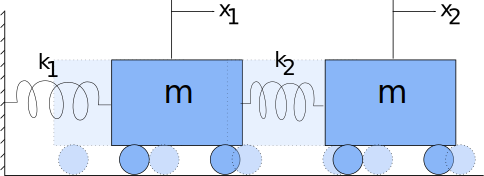
\includegraphics[width=0.6\textwidth]{figs/massSpringDamperSystemCoupled.pdf} 
\caption{Forced vibration with a coupled spring-mass system}
\end{figure}
with $m_1=2$ kg, $k_1 = 4$ N/m, $m_2=1$ kg, $k_2 = 2$ N/m.

\textbf{Solution:}\\
\begin{enumerate}
\item Find the governing equation of the system:\\
The governing equation is:
 \begin{align*}
&m_1x''_1 +\left(k_1+k_2\right)x_1-k_2x_2 = 0\\
&m_2x''_2 +k_2x_2- k_2x_1= 0
\end{align*}
\item Write in differential operator form:
 \begin{align*}
&\left[m_1D^2 +\left(k_1+k_2\right)\right][x_1]-k_2[x_2] = 0\\
&\left[m_2D^2 +k_2\right][x_2]- k_2[x_1]= 0
\end{align*}
\item Identify the linear differential operator:
\begin{itemize}
\item $\mathcal{L}_1=m_1D^2 +\left(k_1+k_2\right)$
\item $\mathcal{L}_2=-k_2$
\item $\mathcal{L}_3=-k_2$
\item $\mathcal{L}_4=m_2D^2 +k_2$
\end{itemize}
\item Eliminate $x_2$:
 \begin{align*}
\left[\mathcal{L}_1\mathcal{L}_4-\mathcal{L}_2\mathcal{L}_3\right][x_1]=0
\end{align*}
we have:
 \begin{align*}
\left[\left(m_1D^2 +\left(k_1+k_2\right)\right)\left(m_2D^2 +k_2\right)-k^2_2\right][x_1]=0
\end{align*}
or
 \begin{align*}
\left[m_1m_2D^4+(m_1k_2+m_2k_1+m_2k_2)D^2+k_1k_2\right)[x_1]=0
\end{align*}
Simplify:
 \begin{align*}
\left[D^4+(\frac{k_2}{m_2}+\frac{k_1+k_2}{m_1})D^2+\frac{k_1k_2}{m_1m_2}\right)[x_1]=0
\end{align*}
We can sub-in the numerical values:
 \begin{align*}
\left(D^4+5D^2 +4\right)[x_1]=0
\end{align*}
we can write in differential form as:
 \begin{align*}
x_1^{(4)}+5x_1^{(2)}+4x_1=0
\end{align*}
we have a 4th order, constant coefficient, homogeneous, and missing term ODE. (we know the solution will have 4 constants)\\

The equation can be solved using the Auxiliary equation:
 \begin{align*}
r_1^{4}+5r_1^{2}+4=0
\end{align*}
We can find: $r^2$ has the roots of -1 and -4. Therefore: $r=\pm i$ and $r=\pm 2i$. Therefore, the solution is:
\begin{equation*}
\boxed{x_1=c_1\cos(t)+c_2\sin(t)+c_3\cos(2t)+c_4\sin(2t)}
\end{equation*}


\item Sub $x_1$ into the governing equation:

 \begin{align*}
x_2&=\frac{1}{k_2}\left[m_1x''_1 +\left(k_1+k_2\right)x_1\right]\\
&=\frac{1}{2}\left[2x''_1 +6x_1\right]=x''_1 +3x_1
\end{align*}
Therefore:
\begin{equation*}
\boxed{x_2=2c_1\cos(t)+2c_2\sin(t)-c_3\cos(2t)-c_4\sin(2t)}
\end{equation*}







\end{enumerate}


\end{exmp}

